\chapter{Grundlagen}

\section{Raspberry Pi}
Der Raspberry Pi wurde von der britischen Raspberry Pi Foundation entworfen um
jungen Menschen den Erwerb von Programmier- und Hardwarekenntnissen zu
ermöglichen. Er ist ein Einplatinencomputer und für wenig Geld verfügbar. Der
Raspberry Pi zeichnet sich durch frei programmierbare Schnittstellen aus um
beispielsweise Sensoren anzuschließen.

Mittlerweile gibt es mehrere Modelle:

\begin{itemize} 
\item Pi Zero 
\item Pi Zero W
\item Pi 1 Modell A
\item Pi 1 Modell A+
\item Pi 1 Modell B
\item Pi 1 Modell B+
\item Pi 2 Modell B
\item Pi 3 Modell B 
\end{itemize}


\section{Sprachen}

\subsection{Python}

\textsc{Bastian Ballmann} \cite{ballmann2012network} stellt die Scriptsprache Python
als eine leicht erlernbare und gut lesbare dynamische Scriptsprache dar. 


\cite{lutz2007einführung}
\subsection{Java}
\cite{abts2015grundkurs}
Java wird als universelle Programmiersprache für eine Vielzahl von Anwendungen
in der industriellen Praxis auf der Client- und insbesondere auf der
Serverseite eingesetzt. Sie dient als Standard für die Entwicklung von Unternehmenssoftware
und Webanwendungen sowie in technische Systeme (Geräte der
Unterhaltungselektronik, der Medizintechnik usw.) eingebettete und mobile
Anwendungen (z. B. Apps auf der Basis des Betriebssystems Android).
Ein hervorstechendes Merkmal von Java ist die Plattformunabhängigkeit, d. h. in
Java programmierte Anwendungen sind ohne Portierung auf nahezu allen
Rechnersystemen lauffähig.
Java hat von den Erfahrungen mit anderen Programmiersprachen wie Smalltalk, C
und C++ profitiert. Wesentliche Konzepte wurden übernommen. Auf allzu
komplexe und fehleranfällige Eigenschaften wurde bewusst verzichtet, um die
Sprache verhältnismäßig einfach und robust halten zu können.
\subsection{SQL}
\cite{schicker2017datenbanken}
Als Zugriffssprache wird SQL (Structured Query Language) verwendet. SQL war zunächst
eine Sprache für den Endbenutzer. Inzwischen dominieren grafische Oberflächen
als Schnittstelle zum Anwender. Als Sprache für den Datenbankprogrammierer hat SQL
dafür eine umso größere Bedeutung erlangt. SQL hat sich, insbesondere seit der ersten
Normierung (SQL1 1987), zur wichtigsten Standardsprache für Datenbanken entwickelt.
Diese erste Norm (im Weiteren als SQL1 Norm bezeichnet) wurde 1992 erheblich erweitert
(SQL2 1992). Die SQL2 Norm ist heute durchgängig implementiert, voll alltagstauglich
und außer für Spezialanwendungen völlig ausreichend. Sie ist daher die Basis dieses
Kapitels.
\subsection{HTML}
\cite{plenk2017angewandte}
Die HypertextMarkup Language, abgekürzt HTML, ist eine textbasierte
Auszeichnungssprache. Das bedeutet, dass HTML beliebige, von Menschen
für Menschen geschrieben Texte strukturiert. Die visuelle Darstellung
der Texte ist nicht Teil der HTML-Spezifikationen und wird durch
den Webbrowser und Gestaltungsvorlagen wie CSS bestimmt.
HTML kennt verschiedene Gliederungsebenen, Absätze und Tabellen
zur Strukturierung digitaler Dokumente. Zusätzlich bietet es Hyperlinks,
Bilder und andere multimediale Inhalte. HTML-Dokumente sind
die Grundlage des World Wide Web und werden von Webbrowsern dargestellt.
Neben den vom Browser angezeigten Inhalten können HTMLDateien
zusätzliche Angaben in Form von Metainformationen enthalten,
z. B. über die im Text verwendeten Sprachen, den Autor oder den zusammengefassten
Inhalt des Textes.
\subsection{PHP}
\cite{pomaska2012webseiten-programmierung}
PHP Hypertext Preprocezor wurde für die Web-Programmierung entwickelt. Die
Sprache orientiert sich an den typischen Aufgaben von Internetanwendungen, das
sind die Übermittlung von Formulardaten, die Anbindung von Datenbanken oder
auch die Erzeugung von Webseiten selbst. Es gibt viele Gründe für den Einsatz
von PHP. Da ist zunächst die weite Verbreitung des Open Source-Projekts mit der
plattformübergreifenden Anwendung auf unterschiedlichen Betriebssystemen zu
nennen. Der Entwickler profitiert von der Verfügbarkeit von Programmbausteinen,
die er in seine Applikation integrieren kann

\subsection{Javascript}
\cite{pomaska2012webseiten-programmierung}
JavaScript ist keinesfalls mit der objektorientierten Programmiersprache Java in
Verbindung zu bringen, obwohl die Syntax der Sprachelemente in vielen Fällen
gleich ist. JavaScript stellt eine objektbasierte Skriptsprache dar und ergänzt die
Funktionalität von Web-Browsern. Der Web-Browser kann den Inhalt einer Webseite
nur statisch abbilden. Durch JavaScript kommt Dynamik in die Seiten. Ohne
eine Seite neu hoch zu laden, werden Elemente durch Benutzereingriffe dynamisch
verändert.

\section{Sensoren}
Der Raspberry Pi besitzt mit den \ac{GPIO} Pins eine Möglichkeit Sensoren anzusteuern. Nach der Dokumentation der Raspberry Pi Foundation\cite{GPIOMode77:online} können die \ac{GPIO} Pins 3.3V liefern und digitale Signale annehmen. Das neue Raspberry Pi 3 Modell hat den gleichen Aufbau der \ac{GPIO} Pins und die gleiche Pinbelegung. Schematisch wird die \ac{GPIO} Schnittstelle wie folgt dargestellt.
\begin{figure}[h]
	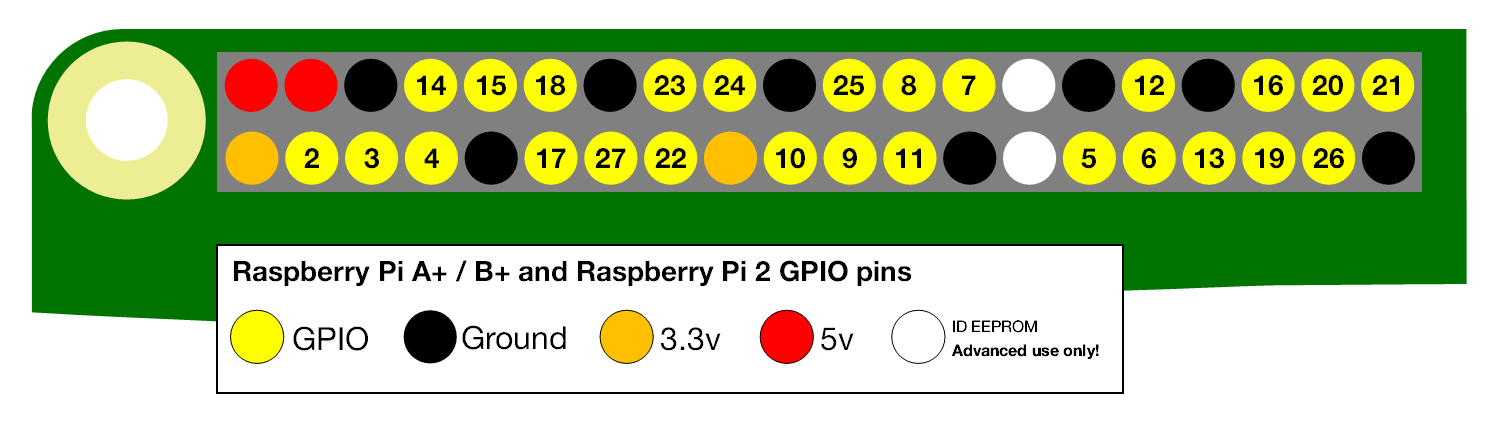
\includegraphics[width=\textwidth]{Bilder/Kapitel2/gpio_pins_pi2.png}
	\caption[Schema GPIO Pins]{Schematische Darstellung der GPIO Pins. Entnommen aus der Raspberry Pi Dokumentation\cite{GPIOMode77:online}.}
	\label{fig:Kapitel2/gpio_pins_pi2.png}
\end{figure}
\noindent
An den vorhandenen 3.3V und 5V Anschlüsse können Sensoren betrieben werden. Dennoch sind nicht alle Sensoren verwendbar. Der Raspberry Pi verfügt nur über die Möglichkeit digitale Signale an den \ac{GPIO} Pins zu verarbeiten. Es werden jedoch neben digitalen auch analoge Sensoren benötigt. Diese können nicht direkt an die Pins angeschlossen werden, aber das Problem wird mit einem \ac{A/D-Wandler} gelöst. \\
Die Erweiterungsplatine RPi-Explorer 700 von Joy-IT \cite{joyitrpi87:online} beinhaltet einen \ac{A/D-Wandler} an dem Analoge Pins angeschlossen werden können. Durch die Erweiterung ist es möglich bis zu vier analoge Sensoren an einem Sensorknoten betrieben werden. \\
Die \ac{GPIO} Schnittstelle unterstützt nur eine maximale Versorgungsspannung von 3.3V, was für die Sensoren ausreichend ist. Durch die Kompatibilität zum Arduino und dem Raspberry Pi können die Sensoren sowohl mit 5V als auch mit 3.3V betrieben werden.
Folgende Sensoren von Allnet\cite{111861pd90:online} werden  im \fullref{Verdrahtung_der_Sensoren} verwendet:
\begin{description}
\item[Temperatur und Luftfeuchtigkeitssensor] \hfill \\
	Der Sensor, KY-015, vom Typ DHT11 kann Temperaturen von 0 bis 50$^\circ$C mit einer Messungenauigkeit von $\pm$ 2$^\circ$C. Die Luftfeuchtigkeit kann im Bereich von 20 bis 95\% ($\pm$ 5\%) gemessen werden. Hierbei handelt es sich um einen digitalen Sensor.  
\item[Flammensensor]\hfill \\
	Der KY-026 besteht aus einer Fotodiode und einem \ac{Poti}. Die Fotodiode kann Wellenlängen im Bereich von etwa 720 - 1100 nm detektieren. Die Diode hat einen Erfassungswinkel von etwa 60$^\circ$. Der \ac{Poti} wird zur Empfindlichkeitseinstellung genutzt, somit kann eine Reichweite von etwa  ein bis sieben Metern abgedeckt werden. Der Sensor besitzt einen "'Digital Out"'-Pin, der high active geschalten wird. Sobald eine Flamme erkannt wird, liegt eine logische 1 auf dem Pin. Der "'Analog Out"'-Pin liefert ein analoges Signal, an welchem bei einer gemessenen Flamme eine niedrige Spannung anliegt.
\item[Lichtschranke]\hfill \\
	Das KY-010 Modul ist eine Lichtschranke, die beim Unterbrechen eine logische 1 an dem digitalen Ausgangspin liefert.
\item[Mikrofon]\hfill \\
	Das Mikrofon, KY-038, hat den gleichen Aufbau wie der Flammensonser. Im Gegensatz zum Flammensensor wird hierbei ein Mikrofonmodul, statt einer Fotodiode genutzt. Die Signale am Digital Out und Analog Out haben die gleiche Funktionalität wie beim Flammensensor. Dieses Modul dient hauptsächlich zur Detektion von kurzen aber lauten Tönen. Ein Anwendungsbeispiel hierfür ist eine Alarmfunktion. Beispielsweise kann das Zerbrechen eines Fensters festgestellt werden.
\item[Lichtsensor]\hfill \\
	Der Lichtsensor KY-018, bestehend aus einem Fotowiderstand, hat bei Dunkelheit einen Widerstand $>$20M$\Omega$ und bei Helligkeit $<$ 80$\Omega$. Damit kann bestimmt werden, ob in einem Zimmer das Licht brennt. Der Lichtsensor liefert ein analoges Signal.
\item[Schocksensor]\hfill \\
	Der Erschütterungssensor liefert eine logische 1 an dem Ausgangspin, falls eine Erschütterung festgestellt wurde. Das dient exemplarisch zur Umsetzung einer Schritterkennung am Boden.
\end{description}
\section{WLAN}
\subsection{Standard}

Die Vernetzung erfolgt über ein Funknetz nach dem WLAN-Standard 802.11n. 

\subsection{Verschlüsselung}
WEP, WPA, WPA2
%%


